\section{Phục dựng cấu trúc từ chuyển động}

SfM là một quy trình nền tảng và quan trọng trong lĩnh vực thị giác máy tính, đóng vai trò then chốt trong việc khôi phục thông tin hình học 3D của một cảnh hoặc đối tượng từ một tập hợp các hình ảnh 2D được chụp từ các góc nhìn khác nhau. Điểm đặc biệt của SfM là khả năng hoạt động hiệu quả ngay cả khi không có thông tin tiên nghiệm về vị trí và hướng của máy ảnh cũng như thứ tự chụp ảnh \cite{Snavely06Photo}. 
Kết quả đầu ra của quy trình SfM thường bao gồm một đám mây điểm 3D thưa biểu diễn cấu trúc hình học của cảnh, tham số nội tại của máy ảnh và đặc biệt là thông tin camera pose chính xác cho từng ảnh đầu vào. Trong phạm vi nghiên cứu luận văn này, SfM có ý nghĩa đặc biệt quan trọng vì nó cung cấp phương pháp để ước lượng camera pose từ tập ảnh 2D ban đầu – thông tin đầu vào thiết yếu cho việc tái tạo mô hình đám mây điểm chi tiết của MVS và việc huấn luyện mô hình tái tạo 3D chi tiết dựa trên học sâu như NeRF sẽ được trình bày ở các phần sau.

Một quy trình SfM điển hình bao gồm nhiều giai đoạn phức tạp, nhưng phổ biến là được phân chia thành 2 giai đoạn chính: Giai đoạn tìm kiếm sự tương ứng và giai đoạn tái tạo 3D \cite{Schonberger16SFMRevisited}, như biểu diễn trong Hình \ref{fig:incre_sfm}.

\begin{figure}[H]
    \centering
    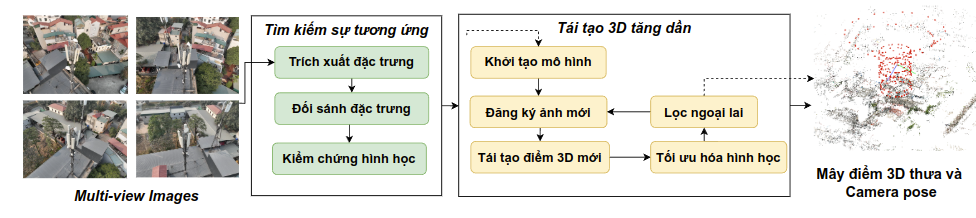
\includegraphics[width=\linewidth]{figures/c3/incremental_sfm.png}
    \caption{Quy trình ước tính camera pose của thuật toán SfM truyền thống.}
    \label{fig:incre_sfm}
\end{figure}

\subsection{Tìm kiếm sự tương ứng}
Mục tiêu của giai đoạn này là phát hiện và xác nhận các điểm ảnh tương ứng trên các ảnh khác nhau trong tập ảnh đầu vào $\mathcal{I} = \{I_i \mid i = 1, \ldots, N_I\}$. Việc xác định đúng các tương ứng này cho phép xây dựng các cặp ảnh có chồng lấp cảnh thực sự và thiết lập các ràng buộc hình học giữa chúng. Các tương ứng được sử dụng để xây dựng một đồ thị quan sát, nơi các đỉnh đại diện cho ảnh và các cạnh đại diện cho mối liên kết hình học giữa các ảnh thông qua các điểm 3D quan sát chung. Độ chính xác của quá trình tìm kiếm tương ứng ảnh hưởng trực tiếp đến chất lượng của việc ước lượng tham số máy ảnh và tái dựng mô hình 3D sau đó. Giai đoạn tìm kiếm sự tương ứng thường bao gồm ba bước chính: (1) Trích xuất đặc trưng, (2) Đối sánh đặc trưng, (3) Kiểm chứng hình học.

\textbf{Trích xuất đặc trưng.} Đối với mỗi ảnh $I_i$, một tập hợp các điểm đặc trưng $\mathcal{F}_{i}=\{(x_{j},f_{j})\}$ được phát hiện tại các vị trí điểm ảnh $x_j = (u, v)$ có cấu trúc đặc trưng nổi bật \cite{McGlone80Manual}. Mỗi điểm đặc trưng này được gắn với một vector mô tả $f_j$ nhằm mã hóa thông tin về vùng ảnh lân cận vị trí đó. Để đảm bảo khả năng đối sánh chính xác giữa các ảnh chụp ở các góc nhìn khác nhau, các đặc trưng và bộ mô tả cần có tính bất biến cao trước các thay đổi về chiếu sáng và phép biến đổi hình học \cite{Tuytelaars08Local}. Ngày nay, các thuật toán trích xuất đặc trưng kinh điển như SIFT \cite{Lowe04Distinctive} và các biến thể của nó, hay gần đây là các đặc trưng được học dựa trên mạng học sâu thường được ưa chuộng và sử dụng trong hầu hết các bài toán vì độ tin cậy và chính xác cao. 

Thuật toán SIFT (Scale-Invariant Feature Transform) là một phương pháp trích xuất đặc trưng hình ảnh được đề xuất bởi David Lowe, được cải tiến vào năm 2004 \cite{Lowe04Distinctive}. SIFT được thiết kế để phát hiện và mô tả các đặc trưng cục bộ trong hình ảnh, đảm bảo tính bất biến đối với thay đổi tỷ lệ, xoay, và một phần đối với thay đổi ánh sáng và góc nhìn. SIFT xây dựng một tháp Gaussian để biểu diễn hình ảnh ở nhiều tỷ lệ khác nhau, từ đó có thể trích xuất ra các điểm đặc trưng có tính bất biến với tỷ lệ. Chính vì vậy các đặc trưng cố định, góc cạnh thường được SIFT ưu tiên trích xuất, minh họa ở Hình \ref{fig:sift_detection}.

\begin{figure}[H]
    \centering
    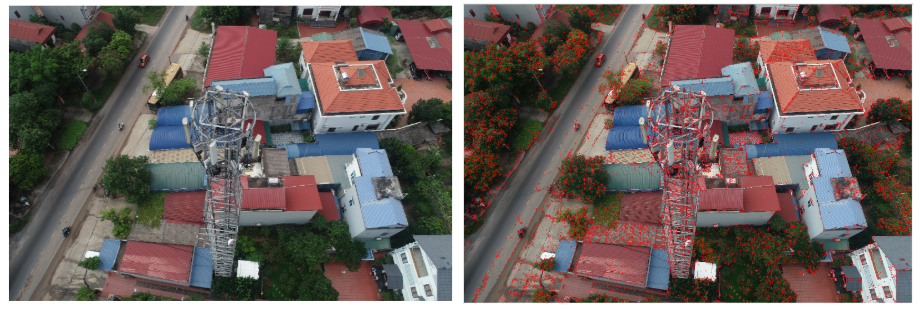
\includegraphics[width=0.9\linewidth]{figures/c2/sift_detection.png}
    \caption{Trích xuất điểm đặc trưng dựa trên SIFT. Các điểm màu đỏ thể hiện điểm đặc trưng quan trọng được phát hiện bởi SIFT. }
    \label{fig:sift_detection}
\end{figure}

\textbf{Đối sánh đặc trưng}. Sau khi phát hiện các đặc trưng của mỗi bức ảnh, bước đối sánh đặc trưng được thực hiện để tìm kiếm các cặp ảnh có khả năng quan sát cùng một điểm trong không gian 3D. Cách tiếp cận đơn giản nhất là duyệt qua tất cả các cặp ảnh và tìm kiếm các cặp đặc trưng có vector mô tả $f_j$ tương đồng nhất giữa chúng. Tuy nhiên, với độ phức tạp tính toán lên tới $O(N_{I}^{2}N_{F_{i}}^{2})$, phương pháp này không khả thi cho các tập ảnh số lượng lớn. Do đó, nhiều kỹ thuật đối sánh hiệu quả và có khả năng mở rộng đã được phát triển để giảm thiểu chi phí tính toán mà vẫn đảm bảo tìm được đủ số lượng đối sánh cần thiết. Kết quả của bước này là một tập hợp các cặp ảnh được khớp nối tiềm năng $\mathcal{C}$ và các cặp đối sánh đặc trưng thô $\mathcal{M}_{ab}$ giữa chúng.

\textbf{Kiểm chứng hình học}. Do việc đối sánh đặc trưng chủ yếu dựa trên sự tương đồng về đặc trưng ngoại hình, tập hợp các đối sánh thô $\mathcal{M}_{ab}$ thường chứa một tỷ lệ đáng kể các cặp sai, gây ảnh hưởng tiêu cực đến kết quả của các bước xử lý sau. Vì vậy, bước kiểm chứng hình học đóng vai trò quan trọng trong việc loại bỏ các đối sánh sai này. Quá trình kiểm chứng được thực hiện bằng cách ước lượng một mô hình biến đổi hình học giữa hai ảnh, nhằm kiểm tra tính nhất quán hình học của các cặp đối sánh thô. Các mô hình thường được sử dụng bao gồm: ma trận homography ($\mathbf{H}$), áp dụng cho trường hợp cảnh phẳng hoặc chuyển động quay; ma trận cơ bản ($\mathbf{F}$) dùng khi các tham số nội tại của máy ảnh chưa được biết; và ma trận cốt yếu ($\mathbf{E}$), sử dụng khi máy ảnh đã được hiệu chuẩn đầy đủ.\cite{Hartley03Multiple}. Vì dữ liệu có chứa ngoại lai, cho nên các phương pháp ước lượng mạnh mẽ như RANSAC \cite{Fischler81RANSAC} hoặc các biến thể của nó được sử dụng để tìm ra mô hình phù hợp nhất được với đa số các đối sánh. Nếu một mô hình hợp lệ được tìm thấy với số lượng cặp đối sánh chính xác đủ lớn, cặp ảnh đó được xem là đã được kiểm chứng hình học, ký hiệu là $\overline{\mathcal{C}}$, và chỉ các đối sánh tốt, ký hiệu là $\overline{\mathcal{M}}_{ab}$ được giữ lại để phục vụ cho các bước tính toán của giai đoạn sau.

Kết thúc giai đoạn tìm kiếm tương ứng, chúng ta thu được đồ thị cảnh với các liên kết hình học đáng tin cậy, làm đầu vào vững chắc cho giai đoạn tái tạo 3D tăng dần sẽ được mô tả ở các phần tiếp theo.

\subsection{Tái tạo tăng dần} 
\label{subsec:incremental_reconstruction} 
    
Quá trình tái tạo cấu trúc 3D thưa trong SfM thường được thực hiện theo ba kiểu quy trình vòng lặp chính bao gồm: quy trình tái tạo tăng dần, quy trình tái tạo toàn cục, quy trình tái tạo kết hợp. Mỗi loại có những ưu, nhược điểm và ứng dụng khác nhau. Trong luận văn này sẽ tập trung giới thiệu về quy trình tái tạo tăng dần, được minh họa trong Hình \ref{fig:incre_sfm}. Đây là một quy trình có tính ổn định cao được sử dụng trong nền tảng COLMAP - một nền tảng mã nguồn mở mạnh mẽ được sử dụng rộng rãi trong lĩnh vực tái tạo 3D.

Sau khi giai đoạn Tìm kiếm sự tương ứng đã thiết lập được đồ thị cảnh với các liên kết hình học đáng tin cậy giữa các cặp ảnh đa góc nhìn, giai đoạn Tái tạo tăng dần bắt đầu được thực hiện để tái tạo thông tin về cấu trúc 3D của cảnh, đối tượng. Mục tiêu của giai đoạn này là xây dựng mô hình hình học 3D của cảnh và ước lượng camera pose một cách tuần tự theo từng vòng lăp. Thuật toán khởi đầu từ một cấu hình nhỏ, có thể là tìm kiếm cặp ảnh có đối sánh cao nhất và dần dần mở rộng bằng cách thêm vào các hình ảnh và điểm 3D mới. Đầu vào chính là đồ thị cảnh đã được kiểm chứng hình học, và đầu ra là một tập hợp các camera pose đã được tối ưu, hiệu chỉnh  $\mathcal{P} = \{P_c \in SE(3)\}$ và một tập hợp các điểm 3D tái tạo $\mathcal{X} = \{X_k \in \mathbb{R}^3\}$ với độ chính xác nhất định dựa trên ngưỡng của chỉ số RE (sai số chiếu lại). Quy trình tái tạo cấu trúc 3D tăng dần bao gồm 2 bước chính: Khởi tạo mô hình và Vòng lặp tái tạo.

\subsubsection{Khởi tạo mô hình }
Quá trình tái tạo tăng dần thường được khởi tạo từ một mô hình hai góc nhìn được lựa chọn cẩn thận từ đồ thị cảnh. Việc chọn cặp ảnh $(I_a, I_b)$ phù hợp để khởi tạo là cực kỳ quan trọng, bởi vì một lựa chọn không tốt ví dụ như đường cơ sở quá ngắn (đường thẳng nối 2 vị trí chụp ảnh), cấu hình hình học suy biến, hoặc ước lượng ma trận F/E không chính xác đều có thể dẫn đến mô hình bị lỗi hoặc không thể phục hồi trong các bước tiếp theo. Các tiêu chí lựa chọn thường bao gồm số lượng đối sánh đặc trưng đủ lớn, các điểm ảnh được phân bố tốt trên cả hai ảnh, và một đường cơ sở phù hợp để đảm bảo phép giao hội đáng tin cậy \cite{Beder06Determining, Snavely08Thesis}.

Vị trí của cặp ảnh khởi tạo trong đồ thị cảnh cũng ảnh hưởng đến chất lượng và hiệu năng của toàn bộ quá trình tái tạo. Khởi tạo từ một vùng dày đặc các ảnh chồng lấn thường mang lại độ chính xác ban đầu cao hơn do có nhiều ràng buộc dư thừa, nhưng cũng có thể làm tăng chi phí tính toán cho các bước tối ưu hóa sau này do mô hình được mở rộng nhanh chóng. Ngược lại, khởi tạo từ vùng thưa hơn có thể giúp giảm thời gian chạy ban đầu nhưng tiềm ẩn rủi ro về độ ổn định của mô hình. Sau khi chọn cặp ảnh khởi tạo, ma trận F hoặc E được phân tích để tìm vị trí, hướng tương đối giữa hai máy ảnh, và các điểm 3D ban đầu được tạo ra bằng phép giao hội từ các đối sánh đặc trưng giữa chúng.

\subsubsection{Vòng lặp tái tạo tăng dần}
Khi mô hình 3D ban đầu đã được thiết lập (bao gồm vị trí, hướng của ít nhất hai máy ảnh và một tập các điểm 3D $\mathcal{X}$), quy trình tái tạo sẽ đi vào một vòng lặp để dần dần mở rộng mô hình bằng cách thêm các ảnh mới. Vòng lặp này thường bao gồm các bước chính sau:

\begin{itemize}
    \item \textbf{Lựa chọn ảnh tiếp theo:} Từ tập các ảnh chưa được liên kết, kiểm tra, hệ thống sẽ lựa chọn một hoặc một vài ảnh "tốt nhất" để thêm vào mô hình ở bước tiếp theo. Tiêu chí lựa chọn rất quan trọng để đảm bảo sự ổn định và chính xác của quá trình tái tạo. Một chiến lược phổ biến là chọn ảnh quan sát được nhiều điểm 3D đã có trong mô hình nhất, vì điều này ảnh hưởng trực tiếp tới độ chính khi xác ước lượng camera pose của ảnh được thêm vào. Các chiến lược phức tạp hơn có thể xem xét cả sự phân bố của các điểm 3D trên ảnh (để tránh các cấu hình PnP suy biến) \cite{Lepetit09EPnP}. Bài báo \cite{Schonberger16SFMRevisited} đề xuất một phương pháp lựa chọn hiệu quả dựa trên việc phân tích đồng thời số lượng và sự phân bố của các điểm 3D nhìn thấy được, cho mỗi ảnh xét duyệt. Việc vừa đảm bảo số lượng điểm 3D quan sát được và phân bố đều trên ảnh sẽ đem lại kết quả tốt hơn cho mô hình.

    \item \textbf{Đăng ký ảnh:} Quá trình đăng ký ảnh đóng vai trò then chốt trong việc mở rộng mô hình 3D từng bước một cách ổn định và chính xác. Bước này nhằm mục tiêu ước lượng camera pose $P_c$ của ảnh mới khi thêm ảnh đó vào mô hình đã có, thông qua việc tận dụng các điểm 3D được tái dựng trước đó và các phép chiếu 2D tương ứng trên ảnh mới.

    Giả sử tại thời điểm hiện tại, hệ thống đã xây dựng được một mô hình 3D tạm thời với tập các điểm 3D \( \mathcal{X} = \{ \mathbf{X}_i \in \mathbb{R}^3 \} \), được quan sát bởi một tập con ảnh đã được đăng ký \( \mathcal{I}_{reg} \subseteq \mathcal{I} \). Với một ảnh mới \( I_{\text{c}} \in \mathcal{I} \setminus \mathcal{I}_{reg} \), mục tiêu của bước đăng ký là tìm "\textit{pose}" của máy ảnh tương ứng với ảnh \( I_{\text{c}} \), biểu diễn dưới dạng ma trận chuyển đổi \( [R \mid \mathbf{t}] \in SE(3) \), trong đó \( R \in SO(3) \) là ma trận xoay và \( \mathbf{t} \in \mathbb{R}^3 \) là vector tịnh tiến.
    
    Để thực hiện điều này, đầu tiên ta tìm kiếm các cặp đối sánh đặc trưng giữa ảnh mới \( I_{\text{c}} \) và các ảnh đã được đăng ký, từ đó ánh xạ đến các điểm 3D đã biết trong mô hình. Kết quả thu được là một tập hợp các cặp tương ứng 2D-3D \( \{ (\mathbf{x}_i, \mathbf{X}_i) \} \), trong đó \( \mathbf{x}_i \in \mathbb{R}^2 \) là vị trí điểm ảnh trong \( I_{\text{c}} \), và \( \mathbf{X}_i \in \mathbb{R}^3 \) là điểm 3D tương ứng đã biết.
    
    Với các cặp tương ứng này, bài toán trở thành một trường hợp cổ điển của bài toán \textit{Perspective-$n$-Point (PnP)}, trong đó ta tìm ma trận \( [R \mid \mathbf{t}] \) sao cho:
    
    \begin{equation}
        \mathbf{x}_i \sim \pi\left( K [R \mid \mathbf{t}] \mathbf{X}_i \right)     
    \end{equation}
    
    trong đó \( K \in \mathbb{R}^{3 \times 3} \) là ma trận thông số nội tại của máy ảnh, và \( \pi(\cdot) \) là phép chiếu từ không gian 3D về mặt phẳng ảnh 2D theo mô hình pinhole.
    
    Để tăng độ bền vững trước nhiễu và các đối sánh sai lệch, việc giải bài toán PnP thường đi kèm với thuật toán \textit{RANSAC}, nhằm loại bỏ các ngoại lai và chỉ giữ lại các cặp đối sánh hình học nhất quán. Khi camera pose ảnh được xác định chính xác, ảnh \( I_{\text{c}} \) sẽ được thêm vào mô hình, trở thành một ảnh đã đăng ký.
    
    \item \textbf{Tạo điểm 3D mới - Phép giao hội:} tạo các điểm 3D mới từ các cặp đối sánh giữa ảnh mới \( I_{\text{c}} \) và các ảnh đã được đăng ký trước đó. Quá trình này được gọi là phép giao hội, bởi nó tìm tọa độ không gian của điểm 3D từ hai hoặc nhiều phép chiếu 2D của điểm đó trên các mặt phẳng ảnh của các ảnh khác nhau.

    Cụ thể, giả sử điểm ảnh \( \mathbf{x}_i^{(1)} \in \mathbb{R}^2 \) trong ảnh \( I_1 \) và điểm ảnh tương ứng \( \mathbf{x}_i^{(2)} \in \mathbb{R}^2 \) trong ảnh \( I_2 \) là các hình chiếu của cùng một điểm 3D \( \mathbf{X}_i \in \mathbb{R}^3 \). Biết được ma trận nội tại \( K \) và ma trận tham số trận ngoại (camera pose) \( [R_1\mid\mathbf{t}_1] \), \( [R_2\mid\mathbf{t}_2] \) của hai máy ảnh tương ứng, ta có thể xây dựng phương trình chiếu:
    \begin{align}
        \lambda_1 \mathbf{x}_i^{(1)} &= K \left[ R_1 \mid \mathbf{t}_1 \right] \mathbf{X}_i \\
        \lambda_2 \mathbf{x}_i^{(2)} &= K \left[ R_2 \mid \mathbf{t}_2 \right] \mathbf{X}_i
    \end{align}
    
    trong đó \( \lambda_1 \), \( \lambda_2 \) là các hệ số tỷ lệ liên quan đến độ sâu. Từ hai phương trình trên, ta có thể xây dựng hệ phương trình tuyến tính hoặc phi tuyến để giải cho tọa độ \( \mathbf{X}_i \). Trong thực tế, vì tồn tại nhiễu trong dữ liệu và sai số nội tại trong phép chiếu, các tia chiếu từ ảnh không cắt nhau chính xác mà thường là chéo nhau trong không gian. Do đó, điểm 3D \( \mathbf{X}_i \) được ước lượng là điểm gần nhất tới hai đường thẳng chiếu, hay còn gọi là điểm tối thiểu hóa khoảng cách tới hai tia.
    
    Một cách tiếp cận phổ biến là sử dụng phương pháp giao hội tuyến tính, dựa trên việc xây dựng ma trận \( A \) từ các phương trình chiếu và giải hệ:
    
    \begin{equation}
        A \mathbf{X}_i = 0    
    \end{equation}
    
    sử dụng thuật toán phân tích trị riêng. Ngoài ra, cũng có thể áp dụng giao hội phi tuyến để tối ưu hóa trực tiếp sai số RE:
    
    \begin{equation}
        \mathbf{RE} = \sum_{j=1}^{n} \left\| \mathbf{x}_i^{(j)} - \pi\left( K [R_j \mid \mathbf{t}_j] \mathbf{X}_i \right) \right\|^2    
    \end{equation}    
    trong đó \( \mathbf{x}_i^{(j)} \) là tọa độ điểm ảnh quan sát điểm 3D \( \mathbf{X}_i \) từ máy ảnh thứ \( j \), và \( \pi(\cdot) \) là hàm chiếu pinhole.
    
    Tuy nhiên, không phải mọi cặp đối sánh đều được sử dụng để giao hội. Để đảm bảo độ chính xác và ổn định, chỉ những đối sánh có góc cơ sở đủ lớn và sai số chiếu lại thấp mới được lựa chọn. Góc cơ sở quá nhỏ dẫn đến giao hội yếu và điểm 3D kém chính xác. Ngoài ra, các điểm có số lần quan sát từ nhiều ảnh khác nhau thường được ưu tiên vì giúp cải thiện độ tin cậy của ước lượng tọa độ.
    
    Kết quả của bước này là mở rộng tập điểm 3D \( \mathcal{X} \) trong mô hình hiện tại bằng cách thêm vào các điểm mới \( \mathbf{X}_i \) được tái dựng từ ảnh mới vừa được đăng ký. Những điểm mới này sẽ tiếp tục được sử dụng trong các bước sau và việc đăng ký các ảnh tiếp theo.

    
    \item \textbf{Tối ưu hóa hình học :} Sau khi các điểm 3D mới được tạo ra thông qua phép giao hội, bước quan trọng tiếp theo là tinh chỉnh toàn bộ mô hình để giảm thiểu sai số RE, và đảm bảo sự nhất quán toàn cục của cả cấu trúc không gian 3D và thông số máy ảnh. Quá trình này được gọi là Tối ưu hóa hình học (BA), và được xem là bước cốt lõi trong các hệ thống SfM. Mục tiêu của Tối ưu hóa hình học (BA)\cite{Triggs00Bundle} là đồng thời tối ưu cả các thông số camera pose \( \{ \mathbf{R}_j, \mathbf{t}_j \} \) của mỗi ảnh \( I_{\text{j}} \), các thông số nội tại (nếu cần) và toạ độ không gian của các điểm 3D \( \{ \mathbf{X}_i \} \), sao cho sai số chiếu lại RE là nhỏ nhất. Với một tập các quan sát 2D \( \mathbf{x}_{ij} \) là ảnh chiếu của điểm 3D \( \mathbf{X}_i \) lên ảnh \( I_{\text{j}} \), bài toán được mô hình hoá thành một bài toán tối ưu phi tuyến:

    \begin{equation}
        \min_{\{ \mathbf{R}_j, \mathbf{t}_j, \mathbf{X}_i \}} \sum_{i,j} \rho\left( \left\| \mathbf{x}_{ij} - \pi\left(K_j [\mathbf{R}_j \mid \mathbf{t}_j] \mathbf{X}_i \right) \right\|^2 \right)    
    \end{equation}
    
    Trong đó:
    \begin{itemize}
        \item \( \pi(\cdot) \): hàm chiếu từ không gian 3D về mặt phẳng ảnh,
        \item \( K_j \): ma trận nội tại của máy ảnh thứ \( j \),
        \item \( \rho(\cdot) \): hàm mất mát, ví dụ hàm Huber để giảm ảnh hưởng của nhiễu và ngoại lai,
        \item \( \| \cdot \| \): chuẩn Euclid thể hiện độ lệch giữa điểm ảnh thực tế và điểm ảnh được chiếu lại từ mô hình.
    \end{itemize}
    
    Quá trình tối ưu này thường sử dụng các thuật toán như Levenberg–Marquardt hoặc Gauss–Newton để giải bài toán phi tuyến với số lượng biến lớn. Nhờ tính chất thưa của bài toán (mỗi điểm 3D chỉ được quan sát bởi một vài máy ảnh), một vài kỹ thuật tối ưu hóa hiệu quả nhằm đơn giản hóa bài toán như sử dụng phân rã Schur \cite{triggs1999bundle} giúp rút gọn số lượng biến cần giải, chỉ tập trung vào phần liên quan đến thông số camera pose.
    
    Trong hệ thống SfM sử dụng chiến lược tái tạo tăng dần, việc thực hiện BA toàn cục sau mỗi lần thêm ảnh là không khả thi do chi phí tính toán cao. Thay vào đó, hệ thống áp dụng BA cục bộ, chỉ tối ưu tập con bao gồm máy ảnh mới được thêm vào và các máy ảnh lân cận có quan sát chung với một tập điểm 3D. Phương pháp này cho phép duy trì hiệu quả tính toán trong khi vẫn đảm bảo độ chính xác hình học của mô hình được xây dựng.
    
    Tóm lại, BA đóng vai trò then chốt trong việc nâng cao độ chính xác của mô hình 3D bằng cách giảm thiểu sai số chiếu lại tổng thể của cả mô hình, đồng thời đảm bảo tính nhất quán giữa các quan sát 2D và cấu trúc không gian 3D tái dựng.
    \item \textbf{Lọc ngoại lai:} Sau các bước trên, đặc biệt là sau quá trình Bundle Adjustment, thuật toán sẽ thực hiện lọc bỏ các điểm 3D không đáng tin cậy. Cụ thể, các điểm có lỗi chiếu lại lớn, không thỏa mãn ràng buộc hình học, hoặc được tạo ra từ phép giao hội với góc nhìn quá hẹp sẽ bị loại bỏ \cite{Snavely08Thesis, Wu13Towards}. Việc này giúp loại bỏ các ước lượng sai lệc, cải thiện chất lượng và độ tin cậy của mô hình.
\end{itemize}

Vòng lặp trên được lặp lại cho đến khi không còn ảnh nào có thể được đăng ký một cách đáng tin cậy hoặc khi đạt được một tiêu chí dừng khác. Kết quả cuối cùng là một mô hình 3D thưa và tập hợp các camera pose đã được tối ưu hóa.
